\chapter{Miscellaneous Topics}

In this chapter I have gathered several sections that were previously part of the main book, but
are either no longer being taught as a regular part of the class, are just for fun, or are
in need of significant revision.  More than anything, this is just a storage location for
sections that might be of interest to curious readers or instructors looking for extra
topics.  Take note that ALL of these sections are incomplete in some way.



\section{Existence and Uniqueness of Solutions to First Order ODEs}
Here are a few fundamental questions about differential equations:
\begin{itemize}
    \item When does the solution to a differential equation exist?
    \item If you find a solution is it the only one?
    \item On what domain does the solution make sense?
\end{itemize}
If we don't know that a solution exists (or worse yet, if we know that it doesn't exist)
then there is no need to go searching for it.  Furthermore, we often solve differential
equations with numerical methods but if the solution doesn't exist then our numerical
method is only giving us computational garbage. 
In this section we present two fundamental theorems discussing these questions for first
order differential equations.  

\begin{thm}[Existence Theorem]\label{thm:existence_uniqueness}
    Suppose that $f(t,y)$ is a continuous function in a rectangle of the form
    \[ \{ (t,y) \, : \, a < t < b \, , \, c < y < d \} \]
    in the $ty$-plane.  If $(t_0,y_0)$ is a point in the rectangle then there exists a
    number $\varepsilon > 0$ ad a function $y(t)$ defined for $t_0 - \varepsilon < t < t_0
    + \varepsilon$ that solves the initial value problem
    \[ \frac{dy}{dt} = f(t,y) \quad y(t_0) = y_0 . \]
\end{thm}
\begin{problem}
    What does theorem \ref{thm:existence_uniqueness} mean?
\end{problem}


\begin{thm}[Uniqueness Theorem]\label{thm:uniqueness}
    Suppose that $f(t,y)$ and $\partial f/\partial y$ are continuous function in a
    rectangle of  the form 
    \[ \{ (t,y) \, : \, a < t < b \, , \, c < y < d \} \]
    in the $ty$-plane.  If $(t_0,y_0)$ is a point in the rectangle and if $y_1(t)$ and
    $y_2(t)$ are two functions that solve the initial value problem 
    \[ \frac{dy}{dt} = f(t,y) \quad y(t_0) = y_0  \]
    for all $t$ in the interval $t_0 - \varepsilon < t < t_0 + \varepsilon$ (for
    $\varepsilon >0$) then
    \[ y_1(t) = y_2(t) \]
    for $t_0 - \varepsilon < t < t_0 + \varepsilon$.  That is, the two solution must be
    identical
\end{thm}
\begin{problem}
    What does theorem \ref{thm:uniqueness} mean?
\end{problem}


\begin{problem}
    A bucket of water has a hole in the bottom, and so the water is slowly leaking out.
    The height of the water in the bucket is thus a decreasing function of time $h(t)$
    which changes according to the differential equation 
    \[ \frac{dh}{dt} = -k\sqrt{h} \]
    where $k$ is a positive constant that depends on the size of the hole in and the
    bucket.  If we start out a bucket with 25cm of water in it, then according to this
    model, will the bucket ever empty?
    \begin{enumerate}
        \item Yes
        \item No
        \item Can't tell with the given information
    \end{enumerate}
\end{problem}
\solution{
Can't tell since the solution isn't guaranteed to exist when $h=0$
}



\begin{problem}
    Based upon observations, Kate developed the differential equation 
    \[ \frac{dT}{dt}= -0.09(T-72) \]
    to predict the temperature in her vanilla chai tea.  In the equation, $T$ represents
    the temperature of the chai in $^\circ F$ and $t$ is time.  Kate has a cup of chai
    whose initial temperature is $110^\circ F$ and her friend has a cup of chai whose
    initial temperature is $120^\circ F$.  According to Kate's model, will there be a
    point in time when the two cups of chai have exactly the same temperature?
    \begin{enumerate}
        \item Yes
        \item No
        \item Can't tell with the given information
    \end{enumerate}
\end{problem}
\solution{No.  If so it would violate uniqueness}



\newpage\section{Bifurcations in First Order Differential Equations}
In this section we will explore the behavior of the equilirium solutions in a differential
equation to changes in a parameter.  In some instances the change in a parameter might
cause the behavior of equilibrium points to change from stable to unstable (or possibly
semi-stable).  It is also possible to {\it spawn} new equilibrium points by changing the
values of parameters. 

It is often the case in real models that parameters are not known with 100\% certainty.
Sometimes the parameters come from scientific measurements, sometimes they are estimated
from data, and sometimes they are just a guess.  If you are in any of these cases with a
first order autonomous differential equation model then you should do a bifurcation
analysis to see how the equilibrium solutions change due to the natural variability in the
parameters.  

\begin{problem}[Fish.net]
    A mathematician at a fish hatchery has been using the differential equation 
    \[ \frac{dP}{dt} = 0.5P\left( 1- \frac{P}{200} \right) \]
    as a model for predicting the number of fish that a hatchery can expect to find in
    their pond.  

    \begin{enumerate}
        \item[(a)] What are the equilibrium points of the mathematician's model.  Discuss their
            stability.  Show the equilibrium points with a plot of $\frac{dP}{dt}$ vs.
            $P$, a phase line, and a slope field.  
        \item[(b)] What does the differential equation predict about the future of the
            fish population for several different initial populations? 
        \item[(c)] Recently the hatchery was bought out by \texttt{fish.net} and the new
            owners are planning to allow the public to catch fish at the hatchery (for a
            fee of course).  This means that the previous differential equation used to
            predict future fish populations needs to modified to reflect this new plan.
            For the sake of simplicity, assume that the managers from \texttt{fish.net}
            are going to allow a constant annual harvest rate $k$.  Which of the four
            modified differential equations makes the most sense to you and why?
            \begin{flalign*}
                & (i) \qquad \frac{dP}{dt} = 0.5 P\left( 1-\frac{P}{200} \right) - k \\
                & (ii) \qquad \frac{dP}{dt} = 0.5 P\left( 1-\frac{P}{200} \right) - kP \\
                & (iii) \qquad \frac{dP}{dt} = 0.5 P\left( 1-\frac{P}{200} \right) - kt\\
                & (iv) \qquad \frac{dP}{dt} = 0.5 P\left( 1-\frac{P-k}{200} \right) 
            \end{flalign*}
        \item[(d)] Using the modified differential equation agreed upon from the previous
            problem, discuss the implications that various choices of $k$ will have on
            future fish populations.  In particular, are there choices of $k$ that change
            the nature or number of the equilibrium points?  Defend your work graphically
            and analytically.
%         \item Find the equilibrium points in terms of the model parameters.
%         \item When are there 2, 1, or 0 equilibrium points?
%         \item Draw a plot with the parameter $h$ on the horizontal axis and the value of
%             the equilibrium point(s) on the vertical axis. Use $M = 1$ and $k = 1$ for
%             simplicity.
    \end{enumerate}
\end{problem}
% \solution{
%     \[ \frac{dP}{dt} = kP(M-P) \]
%     has equilibria $P=0$ and $P=M$ (unstable and stable resp.)
% 
%     For a harvesting model:
%     \[ \frac{dP}{dt} = kP(m-P)-h \]
%     Therefore,
%     \[ 0 = kP(M-P)-h \implies -kP^2 _ kMP - h = 0 \implies P = \frac{-kM \pm \sqrt{k^2M^2
%     - 4kh}}{-2k} \]
%     Plot this in GeoGebra to show the bifurcation.
% 
%     Further analysis: 
%     \begin{itemize}
%         \item When $(kM)^2-4kh<0$ there are no equilibrium points.  In other words, 
%             \[ h>\frac{kM^2}{4} \implies \text{no equilibrium points} \]
%         \item When $(kM)^2-4kh=0$ there is 1 equilibrium point.  In other words, 
%             \[ h=\frac{kM^2}{4} \implies \text{1 equilib. point} P_{eq} =
%             \frac{M}{2} \]
%         \item When $(kM)^2-4kh>0$ there are 2 equilibrium points.  In other words, 
%             \[ h<\frac{kM^2}{4} \implies \text{2 equilibrium points} \]
%     \end{itemize}
% }


\begin{problem}\label{prob:generic_bif}
    For each of the following differential equations demonstrate both graphically and
    analytically the way(s) in which the solutions change as the value of $r$ changes.
    Identify the precise value(s) of $r$ for which there is either a change in the number
    of equilibrium solution(s) or a change in the type of equilibrium solution(s).
    \begin{flalign}
        \frac{dy}{dt} &= (y-3)^2 + r \label{eqn:bif_1} \\
        \frac{dy}{dt} &= y^2 - ry + 1 \label{eqn:bif_2}\\
        \frac{dy}{dt} &= ry + y^3 \label{eqn:bif_3}\\
        \frac{dy}{dt} &= y^6 - 2y^4 + r \label{eqn:bif_4}
    \end{flalign}
\end{problem}

\begin{problem}
    Reconsider differential equation \eqref{eqn:bif_1} from Problem \ref{prob:generic_bif}.  Sketch
    a graph with the value of the equilibrium solution on the vertical axis and the value
    of $r$ on the horizontal axis.  Such a graph is referred to as a ``bifurcation
    diagram.''  Connect what you see in the bifurcation diagram to your
    arguments from Problem \ref{prob:generic_bif}.
\end{problem}

\begin{problem}
    Reconsider differential equation \eqref{eqn:bif_2} from Problem
    \ref{prob:generic_bif}.  Sketch a bifurcation diagram with $r$ on the horizontal axis
    and the value of the equilibrium point on the vertical axis.  Connect what you see in
    this plot to the original discussion in Problem \ref{prob:generic_bif}.
\end{problem}

\begin{problem}
    Consider the differential equation 
    \[ \frac{dy}{dt} = y^2 - ry + r \]
    with unknown parameter $r$.  The bifurcation diagram is shown below.  
\begin{center}
    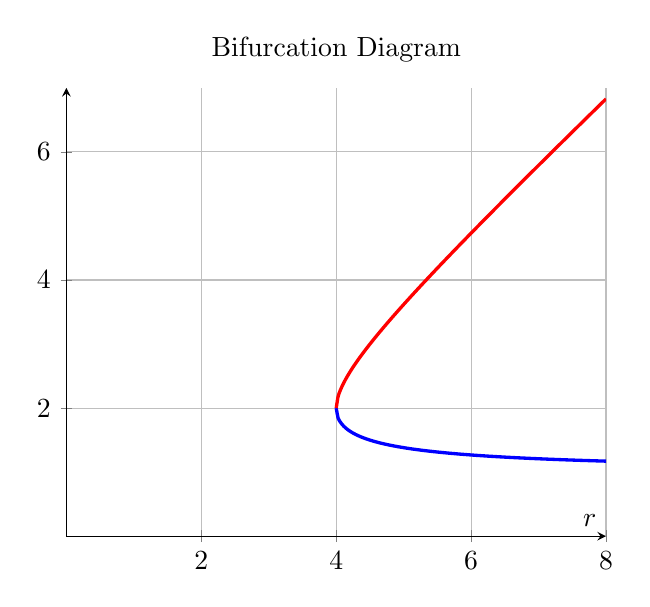
\begin{tikzpicture}
        \begin{axis}[axis lines=center, xlabel={$r$}, title={Bifurcation Diagram}, xmin=0,
            xmax=8, ymin=0, ymax=7, grid]
            \addplot[smooth, very thick, blue, domain=4:8, samples=150] {(1/2)*x-(1/2)*sqrt(x^2-4*x)};
            \addplot[smooth, very thick, red, domain=4:8, samples=150] {(1/2)*x+(1/2)*sqrt(x^2-4*x)};
        \end{axis}
    \end{tikzpicture}
\end{center}
\begin{enumerate}
    \item[(a)] How many equilibrium solutions are there to the differential equation when
        $r<4$? When $r=4$? When $r>4$?
    \item[(b)] Make a plot of $\frac{dy}{dt}$ vs. $y$ assuming that $r > 4$.  Is the blue
        part of the bifurcation diagram stable, unstable or semi-stable?  What about the
        red part?
    \item[(c)] Make a plot of $\frac{dy}{dt}$ vs. $y$ assuming that $r = 4$.  Is the
        single equilibrium point stable, unstable, or semi-stable?
\end{enumerate}
\end{problem}



\newpage\section{Isomorphic Vector Spaces}
What we'll explore in this section is
the following bold claim.
\begin{quote}
    Every vector space of dimension $n$ is {\it geometrically the same} as $\mathbb{R}^n$.
\end{quote}
The consequence of this statement is that, in reality, studying any finite dimensional
vector space is the same as studying the Euclidean spaces $\mathbb{R}^n$.

To make this clear let's look at a few examples.  Consider the vector space $\mathcal{V} =
\mathbb{R}^3$ and the vector space $\mathcal{W} = \mathcal{P}_2$ (polynomials of order 2).
We claim that the set of all polynomials of order 2 is really the same vector space as
$\mathbb{R}^3$.

The standard bases for these two vector spaces are
\[ \mathcal{B}_{\mathcal{V}} = \left\{ \begin{pmatrix} 1\\0\\0\end{pmatrix},
    \begin{pmatrix} 0\\1\\0\end{pmatrix}, \begin{pmatrix}0\\0\\1\end{pmatrix} \right\}
    \quad \text{and} \quad \mathcal{B}_{\mathcal{W}} = \left\{ 1,x,x^2 \right\}. \]
Notice that there is a natural mapping between these two bases:
\[ \begin{pmatrix} 1\\0\\0\end{pmatrix} \leftrightarrow 1 \qquad
    \begin{pmatrix}0\\1\\0\end{pmatrix} \leftrightarrow x \qquad
\begin{pmatrix}0\\0\\1\end{pmatrix} \leftrightarrow x^2. \]
Hence if we have any polynomial $p(x) \in \mathcal{P}_2$ we can use this natural mapping
to find the corresponding vector in $\mathbb{R}^3$.  For a specific example, let's take
the polynomial $p(x) = 3x^2 + 5x - 1$.  Explicitly stating $p(x)$ as a linear combination
of basis vectors from the set $\{1,x,x^2\}$ we see that 
\[ p(x) = -1 (1) + 5(x) + 3(x^2), \]
and hence $p(x)$ maps to
\[ p(x) \mapsto -1 \begin{pmatrix}1\\0\\0\end{pmatrix} + 5
\begin{pmatrix}0\\1\\0\end{pmatrix} + 3 \begin{pmatrix}0\\0\\1\end{pmatrix} =
\begin{pmatrix} -1 \\ 5 \\ 3 \end{pmatrix}. \]
That is to say that the polynomial $p(x) = 3x^2 + 5x-1$ in $\mathcal{P}_2$ is the {\it same
vector} as $\begin{pmatrix}-1\\5\\3\end{pmatrix}$ in $\mathbb{R}^3$.

More generally, the polynomial $a_0 + a_1 x + a_2 x^2 \in \mathcal{P}_2$ is the {\it same
vector} as $\begin{pmatrix}a_0\\a_1\\a_2\end{pmatrix} \in \mathbb{R}^3$.  In this way we
can say that any vector in $\mathcal{P}_2$ has a geometric copy in $\mathbb{R}^3$.  

The words {\it geometrically the same} are not very mathematical.  Instead a mathematician
would use the word {\it isomorphic} meaning {\it same form}.  
\begin{definition}[Isomorphism]
    An {\bf isomorphism} is an invertible mapping between two sets. 
\end{definition}

\begin{definition}[Isomorphic Vector Spaces]
    Two vector spaces are said to be {\bf isomorphic} if there is an isomorphic mapping
    between their bases.
\end{definition}
Since the word {\it isomorphic} means {\it same form} we can loosely describe isomorphic
vector spaces as having the same geometric form -- whatever geometry makes sense in one
vector space makes the same sense in the other.

Let's explore another example using our new terminology.  Consider the vector spaces
$\mathbb{R}^4$ and $M_{2 \times 2}$ (the collection of $2 \times 2$ matrices).  The
standard bases for these vector spaces are
\[ \mathcal{B}_{\mathbb{R}^4} = \left\{ \begin{pmatrix}1\\0\\0\\0\end{pmatrix}\,,\,
    \begin{pmatrix}0\\1\\0\\0\end{pmatrix}\,,\,
    \begin{pmatrix}0\\0\\1\\0\end{pmatrix}\,,\,
    \begin{pmatrix}0\\0\\0\\1\end{pmatrix}\right\} \quad \text{and} \quad
    \mathcal{B}_{M_{2 \times 2}} = \left\{ \begin{pmatrix}1&0\\0&0\end{pmatrix}\,,\,
    \begin{pmatrix}0&1\\0&0\end{pmatrix}\,,\,
    \begin{pmatrix}0&0\\1&0\end{pmatrix}\,,\,
    \begin{pmatrix}0&0\\0&1\end{pmatrix}\right\}
\]
and we note that both of these vector spaces are four dimensional.  
There is a clear natural isomorphism between the two basis sets
\[ 
    \begin{pmatrix}1\\0\\0\\0\end{pmatrix} \leftrightarrow
    \begin{pmatrix}1&0\\0&0\end{pmatrix} \quad
    \begin{pmatrix}0\\1\\0\\0\end{pmatrix} \leftrightarrow
    \begin{pmatrix}0&1\\0&0\end{pmatrix} \quad
    \begin{pmatrix}0\\0\\1\\0\end{pmatrix} \leftrightarrow
    \begin{pmatrix}0&0\\1&0\end{pmatrix} \quad
    \begin{pmatrix}0\\0\\0\\1\end{pmatrix} \leftrightarrow
    \begin{pmatrix}0&0\\0&1\end{pmatrix}.
\]
Hence we see that any $2 \times 2$ matrix has an isomorphic copy in $\mathbb{R}^4$ and the
invertible mapping is
\[ \begin{pmatrix} a & b \\ c & d \end{pmatrix} \leftrightarrow \begin{pmatrix}
    a\\b\\c\\d\end{pmatrix}. \]
More specifically, this means that the matrix $\begin{pmatrix} 2&0\\3&-1\end{pmatrix}$ is
geometrically equivalent (isomorphic) to the vector
$\begin{pmatrix}2\\0\\3\\-1\end{pmatrix}$.



\begin{thm}
    Any vector space of dimension $n$ is isomorphic to $\mathbb{R}^n$.
\end{thm}
\begin{proof}
    Let $\mathcal{V}$ be an $n$ dimensional vector space.  From the definition of
    dimension this means that $\mathcal{V}$ has a basis that contains $n$ vectors.  Let
    the basis $\mathcal{B}_{\mathcal{V}}$ be denoted as 
    \[ \mathcal{B}_{\mathcal{V}} = \{ \bv_1, \bv_2, \ldots, \bv_n\}. \]
    The natural isomorphism between the basis for $\mathcal{V}$ and $\mathbb{R}^n$ is
    therefore
    \[ \bv_1 \leftrightarrow \begin{pmatrix}1\\0\\0\\\vdots\\0\end{pmatrix}, \quad \bv_2
    \leftrightarrow \begin{pmatrix}0\\1\\0\\\vdots\\0\end{pmatrix}, \quad \cdots \quad
\bv_n \leftrightarrow \begin{pmatrix} 0\\0\\\vdots\\0\\1\end{pmatrix}. \]
\end{proof}

\begin{problem}
    Show that $\mathcal{P}_3$ (the space of third order polynomials) is isomorphic to
    $M_{2 \times 2}$.
\end{problem}

Now for some fun.
\begin{problem}
    Let $\mathcal{P}_2$ be the vector space of second order polynomials and let $T$ be a linear
    transformation $T:\mathcal{P}_2 \to \mathcal{P}_1$ that maps a quadratic polynomial to its
    derivative (which of course is linear).  For example, $T(3x^2+5x-1) = 6x+5$.
    \begin{enumerate}
        \item[(a)] Using the natural isomorphism between $\mathcal{P}_2$ and
            $\mathbb{R}^3$ map the polynomial $p(x) = 3x^2 + 5x - 1$ to a vector
            $\bu \in \mathbb{R}^3$. 
        \item[(b)] Using the natural isomorphism between $\mathcal{P}_1$ and
            $\mathbb{R}^2$ map the polynomial $q(x) = 6x+5$ to a vector $\bw \in \mathbb{R}^2$.
        \item[(c)] There is a matrix $A$ such that $A \bu = \bw$.  Find it.
        \item[(d)] Use your answer to part (c) to take the derivative of $p(x) = ax^2 + bx
            + c$.  That is: map $p(x)$ to $\mathbb{R}^3$, apply the matrix transformation
            from part (c), then map your answer from $\mathbb{R}^2$ to $\mathcal{P}_1$.
        \item[(e)] The linear transformation $T:\mathcal{P}_{n} \to \mathcal{P}_{n-1}$
            that takes derivatives of $n^{th}$ order polynomials is equivalent to what
            matrix transformation?
        \item[(f)] \ldots stop and think about this for a second \ldots you just showed
            that taking derivatives of a polynomial is really just a matrix operation
            \ldots mind = blown!
    \end{enumerate}
\end{problem}


\begin{problem}
    Come up with a matrix transformation that has the same action as taking an
    antiderivative.
\end{problem}



\begin{problem}
    True or False: The function $h(t) = 4+3t$ is a linear combination of the functions
    $f(t) = (1+t)^2$ and $g(t) = 2 - t - 2t^2$.  Answer this question by using the fact
    that the polynomial spaces are isomorphic to the Euclidean spaces.
\end{problem}
\solution{
True.  $h(t) = 2f(t) + g(t) = 2(1+2t+t^2) + (2-t-2t^2) = 4 + 3t$
}

% \begin{problem}
%     \begin{itemize}
%             \input{ClickerQuestions/LA.00.17.050}
%     \end{itemize}
% \end{problem}

\begin{problem}
    True or False: The function $h(t) = t^2$ is a linear combination of $f(t) = (1-t)^2$
    and $g(t) = (1+t)^2$. Answer this question by using the fact
    that the polynomial spaces are isomorphic to the Euclidean spaces.
\end{problem}
\solution{False}


\begin{problem}
    The dot product in $\mathbb{R}^2$ is easy remember, but now that we know that
    $\mathbb{R}^2$ is isomorphic to the vector space of all linear functions it is natural
    to ask if there is a natural inner product on $\mathcal{P}_1$ that is analogous to the
    dot product.  Let $p(x) = p_0 + p_1x$ and $q(x) = q_0 + q_1 x$.  Map both $p$ and $q$
    to $\mathbb{R}^2$ via the natural isomorphism and take the dot product.  Does the
    resulting formula give a valid inner product on $\mathcal{P}_1$?  You'll need to check
    the following (according to Definition \ref{def:inner_product}).
    \begin{enumerate}
        \item $\left< p,q\right> = \left<q,p\right>$ for $p,q\in\mathcal{P}_1$?
        \item $\left< p,q+r\right> = \left<p,q\right> + \left<p,r\right>$ for
            $p,q,r\in\mathcal{P}_1$?
        \item $\left<cp,q\right> = c\left<p,q\right>$ for $p,q\in\mathcal{P}_1$ and $c \in \mathbb{R}$?
        \item $\left<p,p\right> \ge 0$ and $\left<p,p\right>=0$ iff $p=0$ for $p \in
            \mathcal{P}_1$.
    \end{enumerate}
\end{problem}



\begin{problem}
    Consider the vector space $M_{2\times2}$ of all $2 \times 2$ matrices along with the
    inner product 
    \[ \left<A,B\right> = \text{trace}(AB^T) = \text{trace}\left( 
        \begin{pmatrix} a_{11} & a_{12} \\ 
                        a_{21} & a_{22} \end{pmatrix} 
        \begin{pmatrix} b_{11} & b_{21} \\
        b_{12} & b_{22} \end{pmatrix} \right) = \text{trace}\left( 
        \begin{pmatrix} a_{11} & a_{12} \\ 
                        a_{21} & a_{22} \end{pmatrix} 
        \begin{pmatrix} b_{11} & b_{12} \\
        b_{21} & b_{22} \end{pmatrix}^T \right)\]
    \[ = \text{trace}\left(
                    \begin{pmatrix} a_{11}b_{11} + a_{12} b_{12} & a_{11}b_{21} +
                        a_{12}b_{22} \\ a_{21}b_{11} + a_{22}b_{12} & a_{21} b_{21} +
                    a_{22} b_{22} \end{pmatrix} \right) \]
    \[ = \left( a_{11}b_{11} + a_{12} b_{12} \right) + \left(  a_{21} b_{21} + a_{22}
    b_{22}\right) \]
    \begin{enumerate}
        \item[(a)] Why is this a natural choice for the inner product between $2 \times 2$ matrices?
        \item[(b)] Complete these sentences: 
            \begin{itemize}
                \item Finding the magnitude of $2 \times 2$ matrices with this inner
                    product is geometrically the
                    same as \underline{\hspace{1in}}.
                \item Projecting a $2 \times 2$ matrix onto another $2 \times 2$ matrix is
                    geometrically the same as \underline{\hspace{1in}}.
                \item Finding angles between $2 \times 2$ matrices is geometrically the
                    same as \underline{\hspace{1in}}.
            \end{itemize}
    \end{enumerate}
\end{problem}


\begin{problem}
    An valid inner product on $\mathcal{P}_1[0,1]$ (the set of all linear functions on the
    interval $[0,1]$) is 
    \[ \left<p,q\right> = \int_0^1 p(x) q(x) dx. \]
    Let $p(x) = p_0 + p_1x$ and $q(x) = q_0 + q_1x$ and observe that 
    \begin{flalign*}
        \int_0^1 p(x) q(x) &= \int_0^1 \left( p_0 + p_1 x \right)\left( q_0 + q_1 x
        \right) dx \\
        &= \int_0^1 \left( p_0 q_0 + (p_0 q_1 + p_1 q_0)x + p_1 q_1 x^2 \right) dx \\
        &= \left( p_0 q_0 x + \frac{(p_0 q_1 + p_1 q_0)}{2} x^2 + \frac{p_1 q_1}{3} x^3
        \right)\Big|_0^1 \\
        &= p_0 q_0 + \frac{1}{2}\left( p_0 q_1 + p_1 q_0 \right) + \frac{1}{3} \left( p_1
        q_1
        \right).
    \end{flalign*}
    While this inner product naturally defines a geometry in the space of all linear
    polynomials it doesn't correspond to our usual Euclidean geometry in the isomorphic
    space $\mathbb{R}^2$. That is, if $\bu, \bw \in\mathbb{R}^2$ then we can map both
    vectors to the vector space $\mathcal{P}_1$ via the natural isomorphism and then take
    the inner product via the integral given above.  Since $\mathbb{R}^2$ and
    $\mathcal{P}_1$ are isomorphic they are {\it geometrically equivalent}, but which
    geometry do we get when we use the integral inner product?
    \begin{enumerate}
        \item[(a)] What is the angle between $\begin{pmatrix}1\\0\end{pmatrix}$ and
            $\begin{pmatrix}0\\1\end{pmatrix}$ in this new geometry?  Are these vectors
            still orthogonal?
        \item[(b)] What is the length of the vector $\begin{pmatrix} 1\\1\end{pmatrix}$ in
            this new geometry?
        \item[(c)] If $\bu \perp \bw$ in Euclidean geometry then what do we know about
            them in this new geometry?
        \item[(d)] If $p \perp q$ in $\mathcal{P}_1$ under the integral inner product,
            what does that mean about their images in $\mathbb{R}^2$ under Euclidean
            geometry?
    \end{enumerate}
\end{problem}

The previous two problems should point out an interesting fact about abstract vector spaces: in
many cases the natural geometry from Euclidean space carries over perfectly to the
abstract setting, and sometimes there is more to be gained in the abstract setting an your
Euclidean intuition doesn't hold.  Remember that abstract vector spaces are not
abstractions for the sake of abstractions.  Instead, the content in this chapter was a
revolutionary leap forward in the understanding of mathematics in the 17th century and it
has allowed us to make many modern mathematical discoveries.  It is no exaggeration to say
that 
\begin{quote}
    much of modern mathematics (and hence modern science) is built upon the idea of an
    abstract vector space.
\end{quote}

In this section we have built up the intuition for isomorphic vector spaces by using the
natural standard bases.  We could have also built up these ideas using any other basis and
everything that we've said thus far is true.  The down side to using non-standard bases,
though, is that the notation and subsequent computations becomes more cumbersome.  For a
more in-depth discussion of these ideas see \cite{Lay}.

\newpage\section{Higher Dimensions are Geometrically Weird}
At this point you have likely come to the conclusion that linear algebra is beautiful but
possibly very hard to visualize.  This is especially true in more than three dimensions.
In this brief section we'll explore a few strange facts about geometry in higher
dimensions.

\begin{problem}
    Let's first recall some basic geometry but in each of the following problems we'll
    intentionally the language of vector spaces.
    \begin{enumerate}
        \item[(a)] If you are standing at the origin on a 1-dimensional Euclidean vector
            space and you reach out $R$ units in each direction, how much {\it volume} do
            you capture? 
            \solution{You are essentially standing on a number line and you're asked to
                find the amount of the number line from $-R$ to $+R$.  Hence, $V_1 = 2R$
            }
        \item[(b)] If you are standing at the origin of a 2-dimensional Euclidean vector
            space and you reach out $R$ units in every direction, how much {\it volume} do
            you capture?
            \solution{You are now on a plane so the geometric object that you form is a
                circle in the plane.  The {\it volume} of the circle is what we would
                typically call the area: $V_2 = \pi R^2$
            }
        \item[(c)] If you are standing at the origin of a 3-dimensional Euclidean vector
            space and you reach out $R$ units in every direction, how much {\it volume} do
            you capture?
            \solution{You are now in the typical 3 dimensions in which we live so the
                geometric object that you form is a sphere.  The {\it volume} of the
                sphere is: $V_3 =\frac{4}{3} \pi R^3$
            }

    \end{enumerate}
\end{problem}

\begin{problem}
    Now let's make a few conjectures.  Let $V_{n,ball}(R)$ be the volume an
    $n$-dimensional ball of radius $R$ and let $V_{n,cube}(R)$ be the volume of an
    $n$-dimensional cube of side length $2R$.  To make this more concrete, in 2D
    $V_{2,ball}(R)$ is the area of a circle of radius $R$ and $V_{2,cube}(R)$ is the area
    of a square with side length $2R$.  In 3D, $V_{3,ball}(R)$ is the volume of a sphere
    with radius $R$ and $V_{3,cube}(R)$ is the volume of a cube with side length $2R$.
    \begin{enumerate}
        \item[(a)] Without any formal computation, approximately how much area does a
            circle inscribed in a square take up?  In other words, what is $V_{2,ball}(R) /
            V_{2,cube}(R)$?  Verify your conjecture with formal computation.
            \begin{figure}[ht!]
                \begin{center}
                    
\begin{tikzpicture}
                        \draw[thick, black] (-1,-1) -- (1,-1) -- (1,1) -- (-1,1) -- cycle;
                        \draw[thick, fill = red, color=red] (0,0) circle(1cm);
                    \end{tikzpicture}
                \end{center}
                \caption{A circle inscribed in a square.  The ratio of the area of the
                    square to the area of the circle is $V_{2,ball}/V_{2,cube}$.}
                \label{fig:circle_square}
            \end{figure}
        \item[(b)] Without any formal computation, approximately how much area does a
            sphere inscribed in a cube take up?  In other words, what is $V_{3,ball}(R) /
            V_{3,cube}(R)$?  Verify your conjecture with formal computation.
        \item[(c)] Make a conjecture for the value of the limit:
            \[ \lim_{n\to\infty} \frac{V_{n,ball}(R)}{V_{n,cube}(R)}. \]
    \end{enumerate}
\end{problem}


In higher dimensions (4D and up) we have a hard time visualizing anything without using
tricks such as color or time-like variables.  
\begin{definition}[Volume of an $n$-Dimensional Ball]
    For the volume of an $n$-dimensional ball we
    have the recursive formula 
    \begin{flalign}
        V_n(R) = \frac{2\pi R^2}{n} V_{n-2}(R)
        \label{eqn:n_ball_volume}
    \end{flalign}
    where $n$ is the dimension and $R$ is the radius.  
\end{definition}

\begin{problem}
    Given that $V_1 = 2R$ and $V_2 = \pi R^2$, use the recursive formula
    \eqref{eqn:n_ball_volume} to verify the formula for the volume of a
    sphere of radius $R$.
    \[ V_3(R) = \underline{\hspace{1in}} \]
\end{problem}
\solution{
    \[ V_3(R) = \frac{2 \pi R^2}{3} \cdot V_1(R) = \frac{2\pi R^2}{3} \cdot \left( 2R
        \right) = \frac{4}{3} \pi R^3 \]
}

\begin{definition}[Volume of an $n$-Dimensional Cube]
    For a cube of $n$ dimensions with side length $2R$ we always have the simple formula
    \begin{flalign}
        V_n(R) = (2R)^n = 2^n R^n.
        \label{eqn:n_cube_volume}
    \end{flalign}
\end{definition}
A moment's reflection reveals that in a one dimension Euclidean vector space the volume of a
cube and the volume of the sphere are the same: $V_{1,ball} = V_{1,cube} = 2R$.  In two dimensions we have 
\begin{flalign*}
    V_{2,square} &= (2R)^2 = 4R^2 \quad \text{and} \\
    V_{2,circle} &= \pi R^2,
\end{flalign*}
which implies that the fraction of the volume of the square filled by the inscribed circle
is
\[ \frac{V_{2,circle}}{V_{2,square}} = \frac{\pi R^2}{4 R^2} =\frac{\pi}{4} \approx 0.785 \]
so the circle fills approximately 78.5\% of the square. Examining Figure
\ref{fig:circle_square} visually should verify that this {\it appears to be} correct.

In three spatial dimension we have
\begin{flalign*}
    V_{3,cube} &= (2R)^3 = 8R^3 \quad \text{and} \\
    V_{3,sphere} &= \frac{4}{3} \pi R^3,
\end{flalign*}
which implies that 
\[ \frac{V_{3,sphere}}{V_{3,cube}} = \frac{\frac{4}{3} \pi R^3}{8 R^3} =
    \frac{\frac{4}{3} \pi}{8} = \frac{\pi}{6} \approx 0.524 \]
so we see that a sphere inscribed in a cube fills up about 52.4\% of the available volume.
These results are summarized in the table below.

\begin{center}
    \begin{tabular}{|c|c|c|c|}
        \hline
        Dimension ($n$) & Volume of a Ball & Volume of a Cube & Ratio: ($V_{n,ball} /
        V_{n,cube}$) \\ \hline \hline
        1 & $2R$ & $2R$ & $1$ \\ \hline
        2 & $\pi R^2$ & $4R^2$ & $\frac{\pi}{4} \approx 0.785$ \\ \hline
        3 & $\frac{4}{3} \pi R^3$ & $8R^3$ & $\frac{\pi}{6} \approx 0.524$ \\ \hline
        4 & $\frac{2\pi R^2}{4} \cdot \left( \pi R^2 \right) = \frac{\pi^2 R^4}{2} $ &
        $16R^4$ & $\frac{\pi^2}{32} \approx 0.308$ \\ \hline
        5 & $\frac{2\pi R^2}{5} \cdot \frac{4}{3} \pi R^3 = \frac{8 \pi^2 R^5}{15}$ &
        $32R^5$ & $\frac{\pi^2}{60} \approx 0.164$ \\ \hline
        6 &  &  &  \\ \hline
        7 &  &  &  \\ \hline
        8 &  &  &  \\ \hline
        $\vdots$ &  &  &  \\ \hline
    \end{tabular}
\end{center}

\begin{problem}
    The previous table shows the ratio $V_{n,ball} / V_{n,cube}$ for dimensions $1$
    through $5$.  Use equations \eqref{eqn:n_ball_volume} and \eqref{eqn:n_cube_volume} to
    complete the computation for dimensions $6$ - $8$ and conjecture the
    value of 
    \[ \lim_{n \to \infty} \frac{V_{n,ball}(R)}{V_{n,cube}(R)}. \]
    Explain the meaning of the limit geometrically (however counterintuitive it is).
\end{problem}
\solution{
    In the limit, the ratio $V_{n,ball}/V_{n,cube}$ goes to zero.  Geometrically this
    means that a ball of radius $R$ takes up less and less space in a cube of side length
    $2R$ as the dimension increases.  In an infinite dimensional space, a ball of radius
    $R$ takes up zero volume.
\begin{center}
    \begin{tabular}{|c|c|c|c|}
        \hline
        Dimension ($n$) & Volume of a Ball & Volume of a Cube & Ratio: ($V_{n,ball} /
        V_{n,cube}$) \\ \hline \hline
        1 & $2R$ & $2R$ & $1$ \\ \hline
        2 & $\pi R^2$ & $4R^2$ & $\frac{\pi}{4} \approx 0.785$ \\ \hline
        3 & $\frac{4}{3} \pi R^3$ & $8R^3$ & $\frac{\pi}{6} \approx 0.524$ \\ \hline
        4 & $\frac{2\pi R^2}{4} \cdot \left( \pi R^2 \right) = \frac{\pi^2 R^4}{2} $ &
        $16R^4$ & $\frac{\pi^2}{32} \approx 0.308$ \\ \hline
        5 & $\frac{2\pi R^2}{5} \cdot \frac{4}{3} \pi R^3 = \frac{8 \pi^2 R^5}{15}$ &
        $32R^5$ & $\frac{\pi^2}{60} \approx 0.164$ \\ \hline
        6 & $\frac{\pi^3}{6} R^6$ & $64R^6$ & $\frac{pi^3}{384} \approx 0.0807$  \\ \hline
        7 & $\frac{16 \pi^3}{105} R^7$ & $128 R^7$  & $\frac{16 \pi^3}{13440} \approx
        0.0369$  \\ \hline
        8 & $\frac{\pi^4}{24} R^8$ & $256 R^8$  & $\frac{\pi^4}{6144} \approx 0.0159$ \\ \hline
        $\vdots$ &  &  &  \\ \hline
    \end{tabular}
\end{center}
}   


\begin{problem}
    If you want to see a cool video about higher dimensional visualization, check out this
    one by {\it 3 Blue 1 Brown:}
    \href{https://youtu.be/zwAD6dRSVyI}{https://youtu.be/zwAD6dRSVyI}.
\end{problem}


\newpage\section{Where Laplace Transforms Come From}
You may have run into Taylor Series in past courses.  The idea is to represent a function
$f(x)$ near the point $x=0$ as an infinite series of power functions:
\begin{flalign}
    f(x) &= \frac{f(0)}{0!}x^0 + \frac{f'(0)}{1!}x^1 + \frac{f''(0)}{2!}x^2 +
    \frac{f^{(3)}(0)}{3!}x^3 + \frac{f^{(4)}(0)}{4!}x^4 +\cdots.
    \label{eqn:TaylorExpanded}
\end{flalign}
More compactly, we can write the Taylor Series as
\begin{flalign}
    f(x) &= \sum_{j=0}^\infty \frac{f^{(n)}(0)}{n!}x^n.
    \label{eqn:TaylorSummation}
\end{flalign}

\begin{problem}
Find the Taylor Series representations for the functions $f(x) = e^x$, $g(x) =
\frac{1}{1-x}$ (for $|x|<1$), and $h(x) = \sin(x)$ all centered at $x=0$.
\begin{flalign*}
    e^x &= \underline{\hspace{3in}} \\
    \frac{1}{1-x} &= \underline{\hspace{3in}} \\
    \sin(x) &= \underline{\hspace{3in}} \\
\end{flalign*}
\end{problem}
\solution{
    \begin{flalign*}
        e^x &= 1 + x + \frac{x^2}{2!} + \frac{x^3}{3!} + \frac{x^4}{4!} + \cdots \\
        \frac{1}{1-x} &= 1 + x + x^2 + x^3 + x^4 + \cdots \\
        \sin(x) &= x - \frac{x^3}{3!} + \frac{x^5}{5!} - \frac{x^7}{7!} + \cdots
    \end{flalign*}
}


The Taylor Series does something else amazing!  In a sense, the coefficients of the Taylor
Series are the DNA of the function.  That is to say: If you know the Taylor coefficients
you know the function and visa versa.

\begin{problem}
    Using problem 1, which function has the following sequence of Taylor coefficients?
    \begin{flalign*}
        &a(n) = \{ 1, 1, 1, 1, 1, \ldots \} \quad \text{corresponds to} \quad
        f(x) = \underline{\hspace{1in}}\\
        &a(n) = \{ 1, 1, \frac{1}{2!}, \frac{1}{3!}, \frac{1}{4!},  \ldots \} \quad \text{corresponds
        to} \quad f(x) = \underline{\hspace{1in}}\\
        &a(n) = \{ 0, 1, 0, -\frac{1}{3!}, 0, \frac{1}{5!}, \ldots \} \quad \text{corresponds
        to} \quad f(x) = \underline{\hspace{1in}}
    \end{flalign*}
\end{problem}
\solution{
\begin{flalign*}
    &\{ 1, 1, 1, 1, 1, \ldots \} \quad \text{corresponds to} \quad
    f(x) = \frac{1}{1-x}\\
    &\{ 1, 1, \frac{1}{2!}, \frac{1}{3!}, \frac{1}{4!},  \ldots \} \quad \text{corresponds
    to} \quad f(x) = e^x\\
    &\{ 0, 1, 0, -\frac{1}{3!}, 0, \frac{1}{5!}, \ldots \} \quad \text{corresponds
    to} \quad f(x) = \sin(x)
\end{flalign*}
}

Hence, if we have a sequence $a(n)$ (and the sequence has some basic
properties\footnote{See any standard Calculus text if you don't recall the necessary
conditions for a Taylor Series to converge.}) then we can associate the sequence with a
function $f(x)$ via the Taylor Series
\[ a(n) \rightsquigarrow f(x) \quad \text{since} \quad \sum_{n=0}^\infty a(n) x^n = f(x). \]

\begin{problem}
    You might be asking yourself ``So what!  Why do I need another way to represent a
    function?''  To answer this question discuss with your partner how you think the
    Taylor sequence ``DNA'' of a function might be a useful tool in this modern age of
    computers (hint).
\end{problem}
\solution{
There are many ways to for a computer to store and understand a transcendental function
line the trigonometric functions and the exponential function.  Your calculator and many
computer programming languages only know these functions by storing their Taylor sequence.
That requires very little computer storage and allows the computer program to calculate
these functions to arbitrary precision.  
}

\subsection*{The Laplace Transform}
Now we're ready to create the Laplace Transform.  The Laplace Transform is the continuous
analog of what we just discussed: If we have a function $a(n)$ we can find a function $f(x)$
such that we replace the sum in the Taylor series with an integral:
\begin{flalign}
    \int_0^\infty a(n) x^n dn = f(x)
    \label{eqn:Laplace_Almost}
\end{flalign}
There are some notational conventions that we have to adjust for:
\begin{enumerate}
    \item We don't typically use $n$ as a continuous variable so we're going to switch it
        to $t$.
    \item We typically don't use the letter ``$a$'' for functions of a continuous variable
        so we'll switch it to $f$.  Then we'll make the right-hand side ``$F$'' so we can
        keep them straight.  The integral now becomes
        \[ \int_0^\infty f(t) x^t dt = F(x) \]
    \item The exponential function $x^t$ is really inconvenient when integrating with
        respect to $t$ so we'll switch it to 
        \[ x^t = e^{\ln(x)t} \quad \implies \quad \int_0^\infty f(t) e^{\ln(x)t} dt = F(x) \]
        (convince yourself that this is the same thing algebraically)
    \item Now the left-hand side will be a function of $\ln(x)$ and the right-hand side
        will be a function of $x$.  This is rather inconvenient so let's make a change of
        variables: replace $\ln(x)$ with $-s$ (the negative sign gives positive
        values when $0<x<1$ and negative values otherwise).  Therefore, the Laplace
        transform is:
        \begin{flalign}
            \boxed{\int_0^\infty e^{-st} f(t) dt = F(s)}
            \label{eqn:LaplaceTransform}
        \end{flalign}
\end{enumerate}

The Laplace transform  associates a function $f(t)$ with a
function $F(s)$ just like the Taylor Series associates a sequence of numbers $a(n)$
with a function $f(x)$:
\[ \boxed{\underbrace{a(n) \rightsquigarrow f(x)}_{\text{Taylor Series}} \quad \text{via} \quad \sum_{n=0}^\infty a(n) x^n = f(x) \qquad \text{and} \qquad
    \underbrace{f(t) \rightsquigarrow F(s)}_{\text{Laplace Transform}} \quad \text{via}
    \quad \int_0^\infty
    e^{-st} f(t) dt = F(s).} \]

Notationally we write the Laplace Transform of $f(t)$ as $\lap{f(t)} = F(s).$  




\newpage\section{Convolutions with Laplace Transforms}
\ldots no content here yet, but I intend to write this up eventually \ldots
